\section{Annexes}
\subsection{Structures des fichiers de log pour \texttt{STAR} et \texttt{Crac}}
\label{annexe:format_log} 
\begin{figure}[H]
  \centering
  \begin{minipage}[b]{0.48\textwidth}
    \centering
    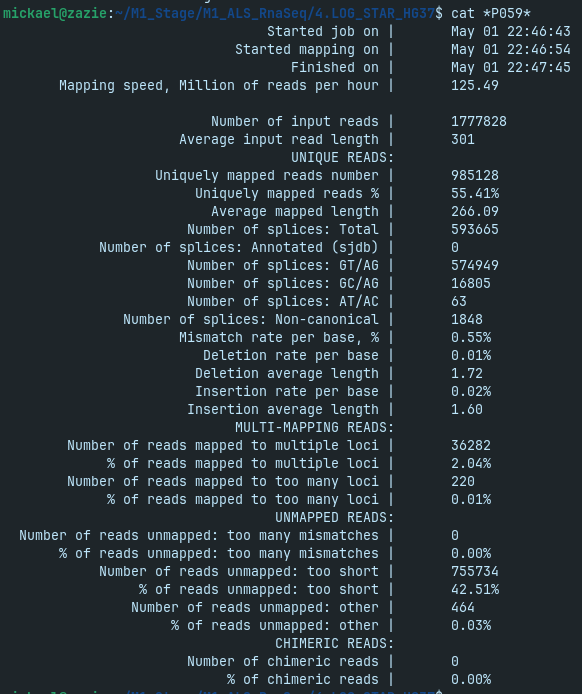
\includegraphics[width=\linewidth]{STAR_log.png}
    \caption*{log d'alignement avec STAR}
  \end{minipage}
  \hfill
  \begin{minipage}[b]{0.48\textwidth}
    \centering
    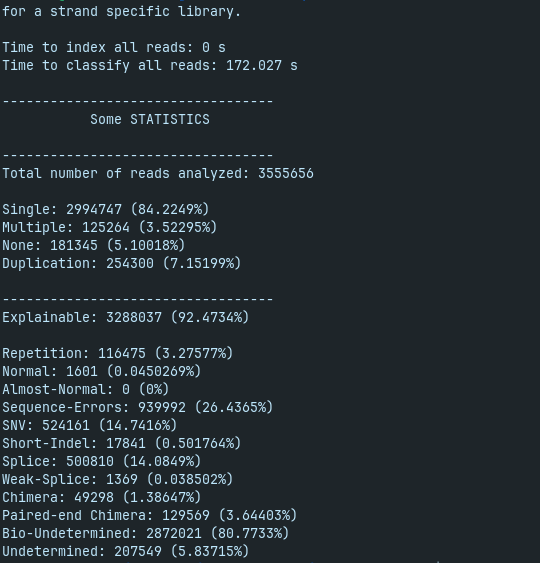
\includegraphics[width=\linewidth]{CRAC_summary.png}
    \caption*{summary généré par CRAC}
  \end{minipage}
  \caption{\underline{Comparaison visuelle des statistiques d’alignement STAR et CRAC.}}
  \label{fig:annexe_star_crac}	
\end{figure}
\newpage
\subsection{Modification du pipeline Snakemake}
\label{annexe:snake_ali}
   \centering
 \begin{lstlisting}[style=makefileStyle,caption={\underline{Règle Snakemake \texttt{aggregateStar} pour l'extraction des statistiques STAR}}]
rule aggregateStar:
    input:
        logs = expand(OUTPUT + "/STAR/results/{sample}/Log.final.out", sample=SAMPLES)
    output:
        csv = OUTPUT + "/STAR/Stats_Log_star.csv"
    shell:
    r"""
    # Headers generation :
    echo "Run,Patient,Type,STAR_Date_Mapping,STAR_Total_reads,\
    STAR_Unique_reads,STAR_Unique_pct,\
    STAR_Multi_reads,STAR_Multi_pct,\
    STAR_No_map_reads,STAR_No_map_pct_sum,STAR_No_map_pct_mismatch,\
    STAR_No_map_pct_tooshort,\
    STAR_No_map_pct_other,\
    STAR_Avg_read_len" > {output.csv}

    # Metrics extraction
    for logfile in {input.logs}; do
        basename=$(basename "$logfile")
        sample=$(echo "$basename" | sed -E 's/.+\/?([^\/]+)_Log.final.out/\1/')
        Run=$(echo "$sample" | cut -d '-' -f1)
        Patient=$(echo "$sample" | cut -d '-' -f2)
        Type=$(echo "$sample" | cut -d '-' -f3 | cut -d '.' -f1)

        Ext() {
            grep "$1" "$logfile" | cut -d '|' -f2 | tr -d ' ' | tr -d '%' || echo "0"
        }
        STAR_Date_Mapping=$(Ext "Finished on")
        STAR_Total_reads=$(Ext "Number of input reads")
        STAR_Unique_reads=$(Ext "Uniquely mapped reads number")
        STAR_Unique_pct=$(Ext "Uniquely mapped reads %")
        ...
        echo "$Run,$Patient,$Type,$STAR_Date_Mapping,$STAR_Total_reads,\
        $STAR_Unique_reads,$STAR_Unique_pct,\
        $STAR_Multi_reads,$STAR_Multi_pct,\
        $STAR_No_map_reads,$STAR_No_map_pct_sum,$STAR_No_map_pct_mismatch,\
        $STAR_No_map_pct_tooshort,$STAR_No_map_pct_other,\
        $STAR_Avg_read_len" >> {output.csv}
    done
    """
\end{lstlisting}

